\documentclass[uplatex,11pt,dvipdfmx,aspectratio=169,unicode,t]{beamer}

% 和文用
\usepackage[utf8]{inputenc}
\usepackage{bxdpx-beamer}
\usepackage{pxjahyper}
\usepackage{minijs} % 和文用
%\usefonttheme{serif}
\renewcommand{\kanjifamilydefault}{\gtdefault} % 和文用
\usepackage{mathtools}
\usepackage{amssymb}
\usepackage{epic,eepic}
\usepackage{color}
\usepackage{caption}
\usepackage{amsmath}
\usepackage{amsthm}
\usepackage{graphicx}
\usepackage[subrefformat=parens]{subcaption}
\usepackage{overpic}
\usepackage{tikz}
\usetikzlibrary{intersections, calc, arrows.meta}
\usepackage[normalem]{ulem}
\usepackage[english]{babel}
\usepackage{media9}
\usepackage{ascmac}
\usepackage{url}
\usepackage{paralist}

% スライドの見た目
\usetheme[
    block=fill, % ブロックに背景をつける
    progressbar=foot, % 各スライドの下にプログレスバー
    numbering=fraction % 合計ページ数を表示
]{metropolis}
%\setbeamercolor{structure}{fg=blue}
\usefonttheme{professionalfonts} % 数式のフォント設定
\setbeamertemplate{frametitle}[default] % フレームタイトルの色(?)
\setbeamertemplate{navigation symbols}{} % プログレスバーを非表示
\setbeamercovered{transparent} % 好みに応じてどうぞ(?)
\setbeamertemplate{footline}[page number] % ページ下部にページ番号を表示
\setbeamerfont{footline}{size=\normalsize,series=\bfseries} %
\setbeamercolor{footline}{fg=black,bg=black} % footlineの色?

% ブロックの色
\setbeamercolor{block title} % ブロックのタイトル部分の色
{fg=black, bg=white!80!black} % fg: 文字色, bg: 背景色
\setbeamercolor{block body} % ブロックの中身の色
{fg=black, bg=black!10!white} % fg: 文字色, bg: 背景色

% ページ番号
\setbeamerfont{frame numbering}{size=\large}

% 図表のキャプション設定
\renewcommand{\figurename}{}
\renewcommand{\tablename}
%\newcommand{\backupbegin}{
%   \newcounter{framenumberappendix}
%   \setcounter{framenumberappendix}{\value{framenumber}}
%}
%\newcommand{\backupend}{
%   \addtocounter{framenumberappendix}{-\value{framenumber}}
%   \addtocounter{framenumber}{\value{framenumberappendix}}
%}

% フォント基本設定
\usepackage[T1]{fontenc}%8bit フォント
\usepackage{textcomp}%欧文フォントの追加
\usepackage[utf8]{inputenc}%文字コードをUTF-8
\usepackage{otf}%otfパッケージ
%\usepackage{lxfonts}%数式・英文ローマン体を Lxfont にする
%\usepackage{bm}%数式太字
%%%%%%%%%%
\allowdisplaybreaks[4]
\setbeamertemplate{enumerate items}[default]

% 目次のフォントサイズ
\setbeamerfont{section number projected}{size=\normalsize}
\setbeamerfont{section in toc}{size=\normalsize}
\setbeamerfont{subsection number projected}{size=\footnotesize}
\setbeamerfont{subsection in toc}{size=\footnotesize}

% % セクションページの設定
% \makeatletter
% \setbeamertemplate{section page}{
%     \centering
%     \begin{minipage}{\linewidth}
%         \raggedright
%         \usebeamercolor[fg]{section title}
%         \usebeamerfont{section title}
%         \insertsectionhead\\[-1ex]
%         \usebeamertemplate*{progress bar in section page}
%         \par
%         \ifx\insertsubsectionhead\@empty\else%
%         \usebeamercolor[fg]{subsection title}%
%         \usebeamerfont{subsection title}%
%         \insertsubsectionhead
%         \fihttps://ja.overleaf.com/project/643cfee13796af4f26269008
%     \end{minipage}
%     \par
%     \vspace{\baselineskip}
% }
% \makeatother

% \metroset{sectionpage=simple} % セクションページの設定その2

% 数式の定義環境
\captionsetup{compatibility=false}
\setbeamertemplate{theorems}[numbered]
\newtheorem{dfn}{Definition}
\newtheorem{thm}{Theorem}
\newtheorem{prop}{Proposition}
\newtheorem{lem}{Lemma}
\newtheorem{cor}{Corollary}
\newtheorem{rmk}{Remark}
\newtheorem{ex}{Example}
\newtheorem{claim}{Claim}
\def\co{\colon\thinspace}

% 数式番号の設定
\numberwithin{equation}{section}
% 参照する数式のみナンバリングする
\mathtoolsset{showonlyrefs=true}

% コマンドの設定
\newcommand{\BC}{\mathbb{C}}
\newcommand{\BE}{\mathbb{E}}
\newcommand{\BK}{\mathbb{K}}
\newcommand{\BN}{\mathbb{N}}
\newcommand{\BP}{\mathbb{P}}
\newcommand{\BR}{\mathbb{R}}
\newcommand{\BV}{\mathbb{V}}
\newcommand{\BZ}{\mathbb{Z}}
\newcommand{\CC}{\mathcal{C}}
\newcommand{\CD}{\mathcal{D}}
\newcommand{\CH}{\mathcal{H}}
\newcommand{\CN}{\mathcal{N}}
\newcommand{\CO}{\mathcal{O}}
\newcommand{\CR}{\mathcal{R}}
\newcommand{\CS}{\mathcal{S}}
\newcommand{\mf}[1]{\mathfrak{S}}
\newcommand{\mr}[1]{\mathrm{#1}}
\newcommand{\mb}[1]{\mathbf{#1}}
\newcommand{\tr}[1]{\textrm{#1}}
\newcommand{\tb}[1]{\textbf{#1}}
\newcommand{\ts}[1]{\textsf{#1}}
\newcommand{\ip}[1]{\left \langle #1 \right \rangle}
\newcommand{\diff}[2]{\frac{d}{d#1} {#2}}
\newcommand{\bs}[1]{\boldsymbol{#1}}
\newcommand{\ti}[1]{\textit{#1}}
\newcommand{\pd}[1]{\frac{\partial}{\partial#1}}
\newcommand{\pdd}[1]{\frac{{\partial}^{2}}{{\partial}^{2}#1}}
\newcommand{\1}{\bs{1}}
\newcommand{\0}{\bs{0}}
\newcommand{\GL}[2]{GL_{#1}{#2}}
\newcommand{\st}{\mathrm{\ s.t.\ }}
\newcommand{\id}[1]{\mathrm{id}_{#1}}
\newcommand{\norm}[1]{\|#1\|}

\DeclareMathOperator*{\argmin}{argmin}
\DeclareMathOperator*{\argmax}{argmax}
\DeclareMathOperator*{\rank}{rank}
\DeclareMathOperator*{\diag}{diag}

\newcommand{\showmovie}[1]{\centering\includemedia[
    activate=pageopen,
    deactivate=pageclose,
    width=30pt, height=30pt,
    addresource=#1,
    flashvars={
        src=#1
        &loop=true
        &autoPlay=false
    }
    ]{}{StrobeMediaPlayback.swf}
}

% セクションごとの目次ページの設定
\AtBeginSection[]{
    \begin{frame}\frametitle{Outline}
        \tableofcontents[currentsection]
    \end{frame}
}

\title{PRML輪読会\\線形回帰モデル (3.1.1 節 -- 3.1.2 節)}
\author{鈴木拓己}
\institute{}
\date{\today}

\begin{document}

\begin{frame}[plain]
    \titlepage
\end{frame}

\begin{frame}\frametitle{Outline}
    \tableofcontents
\end{frame}

\section{線形基底関数モデル}

\begin{frame}{回帰分析の問題設定および線形回帰モデルの概要}
    訓練データ: $(\bs{x}_{1}, t_{1}),\ldots,(\bs{x}_{N}, t_{N}),\ \bs{x}_{i} \in \BR^{D},\ t_{i} \in \BR.$
    \begin{equation}
        t = \underset{\text{function}}{y(\bs{x})} + \underset{\text{r.v.: error}}{\varepsilon} \quad \longrightarrow \quad \text{関数}\ y\ \text{を推定}
    \end{equation}
    \vspace{-11pt}
    \begin{itemize}
        \item 線形回帰モデル: 入力変数 (に対する非線形変換) の\underline{線形結合}により $t$ を予測
        \begin{itemize}
            \item[-] 線形結合のパラメータ $\bs{w}$ に関しては線形 $\longrightarrow$ 解析が容易
            \item[-] 入力変数に関しては非線形 $\longrightarrow$ モデルの表現力が高い
        \end{itemize}
        \item 回帰モデルの構成法
        \begin{itemize}
            \item[-] 関数 $y \colon \BR^{D} \ni \bs{x} \longmapsto t \in \BR$ を直接構成
            \begin{itemize}
                \item[*] 最も単純なアプローチ
            \end{itemize}
            \item[-] 予測分布 $p(t \mid \bs{x})$ をモデル化
            \begin{itemize}
                \item[*] 実変数に対しては,損失関数として二乗損失関数を選ぶのが一般的であり,\\このとき最適解は $\BE[t \mid \bs{x}]$ となる (1.5.5 節)
            \end{itemize}
        \end{itemize}
    \end{itemize}
    線形回帰モデルは解析的に扱いやすく,より洗練されたモデルの基礎として重要
\end{frame}

\begin{frame}{最も単純な線形回帰モデル}
    \begin{itembox}[c]{最も単純な線形回帰モデル}
        \vspace{-11pt}
        \begin{equation}
            y(\bs{x},\bs{w}) = w_{0} + w_{1}x_{1} + \cdots + w_{D}x_{D}, \quad \text{where} \quad \bs{x} = (x_{1},\ldots,x_{D})^{\top} \in \BR^{D}.
        \end{equation}
    \end{itembox}
    \vspace{-22pt}
    \begin{itemize}
        \item 単に\underline{線形回帰} (linear regression) と呼ばれる
        \item パラメータ $w_{0},\ldots,w_{D}$ に関して線形
        \item 入力変数 $x_{i}$ に関しても線形であるため,表現力に乏しい
    \end{itemize}
    $\longrightarrow$ 入力変数に関して非線形な関数の線形結合を考え,モデルのクラスを拡張
\end{frame}

\begin{frame}{線形基底関数モデル}
    \begin{itembox}[c]{線形基底関数\footnote{\url{https://ja.wikipedia.org/wiki/\%E5\%9F\%BA\%E5\%BA\%95\%E9\%96\%A2\%E6\%95\%B0}}モデル}
        \vspace{-11pt}
        \begin{equation} \label{eq:linear basis function model}
            y(\bs{x},\bs{w}) = \underset{\text{bias項}}{\underline{w_{0}}} + \sum_{j=1}^{M-1} w_{j}\phi_{j}(\bs{x}), \quad \text{where} \quad \bs{x} = (x_{1},\ldots,x_{D})^{\top} \in \BR^{D}.
        \end{equation}
        \vspace{-11pt}
        \begin{itemize}
            \item $M$: モデルの表現力を制御するハイパーパラメータ
            \item $\phi_{j}$: \underline{基底関数} (basis function)
            \item 基底関数からなる\underline{特徴写像} (feature map) $\bs{\phi}$ により,入力 $\bs{x}$ を\underline{特徴空間} (feature space) へ写像:
            \vspace{-5.5pt}
            \begin{equation}
                \bs{\phi} \colon \BR^{D} \ni \bs{x} \longmapsto \bs{\phi}(\bs{x}) = (\phi_{1}(\bs{x}),\ldots,\phi_{M-1}(\bs{x}))^{\top} \in \BR^{M-1}
            \end{equation}
        \end{itemize}
    \end{itembox}
    \begin{itemize}
        \vspace{-22pt}
        \item $\phi_{0}(\bs{x}) \coloneqq 1$ とすれば,式 \eqref{eq:linear basis function model} は $y(\bs{x},\bs{w}) = \sum_{j=0}^{M-1} w_{j}\phi_{j}(\bs{x}) = \bs{w}^{\top}\bs{\phi}(\bs{x})$.
    \end{itemize}
\end{frame}

\begin{frame}{線形基底関数モデルの例: 多項式回帰}
    \begin{ex}[1変数多項式回帰]
        データ $(x,t) \in \BR \times \BR$ に対して,$\phi_{j}(x) \coloneqq x^{j}$ とおくと,
        \begin{gather}
            \bs{\phi} \colon \BR \ni x \longmapsto (1,x,x^{2},\ldots,x^{M-1})^{\top} \in \BR^{M},\\ 
            y(x,\bs{w}) = w_{0} + w_{1}x + w_{2}x^{2} + \cdots + w_{M-1}x^{M-1}.
        \end{gather}
    \end{ex}
    \begin{ex}[多変数多項式回帰 (e.g. $D=2$)]
        データ $(\bs{x},t) = ((x_{1},x_{2}),t) \in \BR^{2} \times \BR$ に対して,$\phi_{k,\ell} \coloneqq x_{1}^{k}x_{2}^{\ell}$ とおくと,
        \begin{gather}
            \bs{\phi} \colon \BR^{2} \ni \bs{x} \longmapsto (1,x_{1},x_{2},x_{1}x_{2},\ldots,x_{1}^{M_{1}-1}x_{2}^{M_{2}-1})^{\top} \in \BR^{M_{1}M_{2}},\\
            y(\bs{x},\bs{w}) = w_{0,0} + w_{1,0}x_{1} + w_{0,1}x_{2} + w_{1,1}x_{1}x_{2} + \cdots w_{M_{1}-1,M_{2}-1}x_{1}^{M_{1}-1}x_{2}^{M_{2}-1}.
        \end{gather}
    \end{ex}
\end{frame}

\begin{frame}{その他の基底関数の例 (1変数の場合)}
    \begin{itemize}
        \item スプライン関数\footnote{\url{https://ja.wikipedia.org/wiki/\%E3\%82\%B9\%E3\%83\%97\%E3\%83\%A9\%E3\%82\%A4\%E3\%83\%B3\%E6\%9B\%B2\%E7\%B7\%9A}}
        \begin{itemize}
            \item[-] 多項式では入力空間のある領域の変化が他のすべての領域に及んでしまう
            \item[-] \underline{入力空間を分割}し,各領域で区分的に多項式をあてはめることにより解決できる
        \end{itemize}
        \item ガウス型基底関数 (動径基底関数, RBF\footnote{\url{https://ja.wikipedia.org/wiki/\%E6\%94\%BE\%E5\%B0\%84\%E5\%9F\%BA\%E5\%BA\%95\%E9\%96\%A2\%E6\%95\%B0}}の例)
        \begin{equation}
            \phi_{j}(x) = \exp{\left\{-\frac{(x-\mu_{j})^{2}}{2s^{2}}\right\}} \propto \CN(\mu_{j},s^{2}).
        \end{equation}
        \item シグモイド基底関数
        \begin{equation}
            \phi_{j}(x) = \sigma\left(\frac{x-\mu_{j}}{s}\right), \quad \text{where} \quad \underset{\text{logistic sigmoid function}}{\underline{\sigma(a) = \frac{1}{1+\exp(-a)}}}.
        \end{equation}
    \end{itemize}
\end{frame}

\begin{frame}{その他の基底関数の例 (1変数の場合)}
    (左) 多項式関数 (中央) ガウス型基底関数 (右) シグモイド基底関数
    \begin{figure}
        \centering
        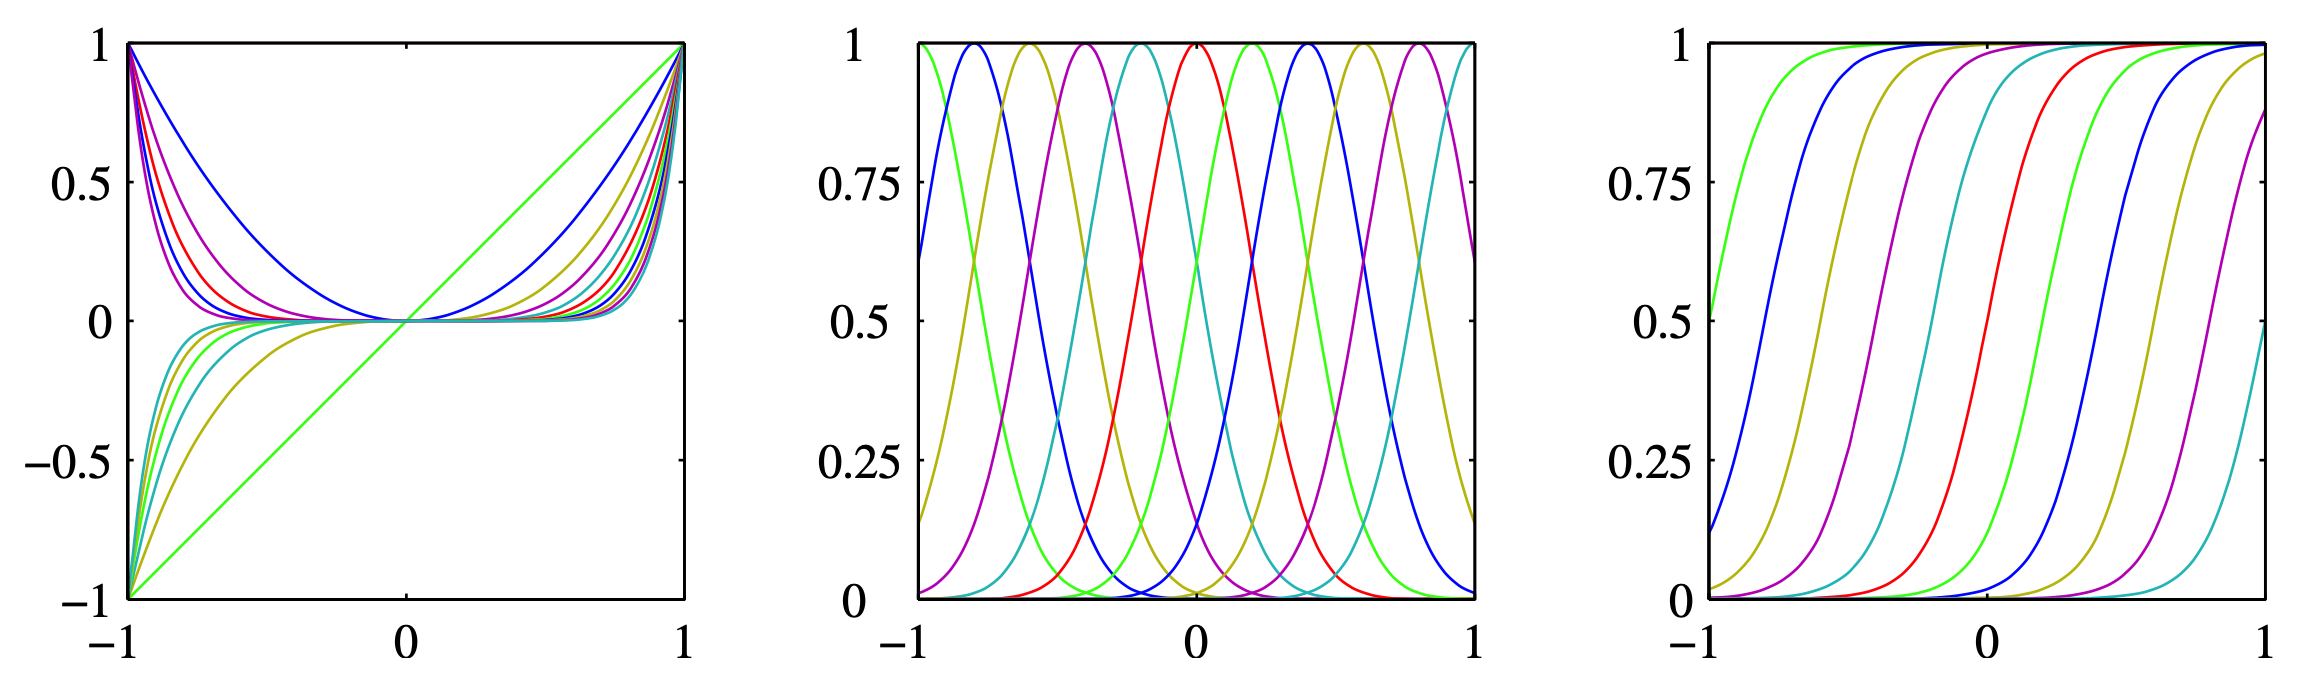
\includegraphics[height=4cm]{prml_fig_3-1.png}
        \caption{基底関数の例}
        \label{fig:3.1}
    \end{figure}
\end{frame}

\begin{frame}{その他の基底関数の例 (1変数の場合)}
    \begin{itemize}
        \item $\tanh$ 関数
        \begin{itemize}
            \item[-] 下記の式変形より,ロジスティックシグモイド関数の線形結合と等価 ($\longrightarrow$ 演習 3.1)
        \end{itemize}
        \begin{align} \label{eq:tanh}
            \begin{aligned}
                \tanh(a) &= \frac{\exp(a) - \exp(-a)}{\exp(a) + \exp(-a)} = \frac{1 - \exp(-2a)}{1 + \exp(-2a)} \\
                &= \frac{2}{1 + \exp(-2a)} - \frac{1 + \exp(-2a)}{1 + \exp(-2a)} = 2\underline{\sigma(2a)} - 1.
            \end{aligned}
        \end{align}
        \item フーリエ基底関数
        \begin{itemize}
            \item[-] 様々な周波数の $\sin$ 関数,$\cos$ 関数による級数展開 (cf.フーリエ級数展開)
        \end{itemize}
        \item ウェーブレット基底関数\footnote{\url{https://ja.wikipedia.org/wiki/\%E3\%82\%A6\%E3\%82\%A7\%E3\%83\%BC\%E3\%83\%96\%E3\%83\%AC\%E3\%83\%83\%E3\%83\%88}}
        \begin{itemize}
            \item[-] フーリエ基底では周波数ごとに定まる基底関数は入力空間において無限に広がる
            \item[-] ウェーブレット基底は入力空間でも周波数領域でも局所的
            \item[-] 詳細は長くなりそうなので,定義と簡単な例のみ確認 (次ページ以降)
        \end{itemize}
    \end{itemize}
\end{frame}

\begin{frame}{その他の基底関数の例 (1変数の場合)}
    \begin{dfn}[ウェーブレット基底]
        関数 $\psi \in L^{2}(\BR) = \{f \colon \BR \rightarrow \BC \mid \int_{\BR} |f(x)|^{2} dx < \infty\}$ に対し,関数 $\psi_{m,n}$ を
        \begin{equation}
            \psi_{m,n}(t) = 2^{m/2} \psi(2^{m}t - n), \quad m \in \BZ, \quad n \in \BZ
        \end{equation}
        で定義する.関数列 $\{\psi_{m,n}\}_{m \in \BZ, n \in \BZ}$ が $L^{2}(\BR)$ において基底\footnote{すなわち,$\forall f \in L^{2}(\BR)$ に対して,$f = \sum_{m \in \BZ} \sum_{n \in \BZ} \ip{f,\psi_{m,n}} \psi_{m,n}$.}をなすとき,$\psi_{m,n}$ を\underline{ウェーブレット},$\psi$ をその\underline{マザーウェーブレット},$\{\psi_{m,n}\}_{m \in \BZ, n \in \BZ}$ を\underline{ウェーブレット基底}という.ウェーブレット基底 $\{\psi_{m,n}\}_{m \in \BZ, n \in \BZ}$ が正規直交条件
        \begin{equation}
            \ip{\psi_{m,n},\psi_{k,\ell}} = \int_{\BR} \psi_{m,n}(t) \overline{\psi_{k,\ell}(t)} dt = \delta_{mk}\delta_{n\ell}
        \end{equation}
        を満たすとき,$\{\psi_{m,n}\}_{m \in \BZ, n \in \BZ}$ を\underline{正規直交ウェーブレット基底}という.
    \end{dfn}
\end{frame}

\begin{frame}{その他の基底関数の例 (1変数の場合)}
    \begin{ex}[直交ウェーブレットの例: Haar ウェーブレット\footnote{\url{https://ja.wikipedia.org/wiki/\%E3\%83\%8F\%E3\%83\%BC\%E3\%83\%AB\%E3\%82\%A6\%E3\%82\%A7\%E3\%83\%BC\%E3\%83\%96\%E3\%83\%AC\%E3\%83\%83\%E3\%83\%88}}]
        マザーウェーブレット $\psi$ を
        \begin{equation}
            \psi(t) = \begin{dcases}
                1, & 0 \le t < 1/2, \\
                -1, & 1/2 \le t < 1, \\
                0, & \text{otherwise},
            \end{dcases}
        \end{equation}
        で定めると,$\{\psi_{m,n}\}_{m \in \BZ, n \in \BZ}$ は直交ウェーブレットとなる.
    \end{ex}
    Haar ウェーブレットのグラフは次ページ.\\
    他にもいろいろな直交ウェーブレットがある (気になる人はpdf\footnote{\url{http://wwwcs.ce.nihon-u.ac.jp/lab/moritaleb224w.pdf}}を参照してください).
\end{frame}

\begin{frame}{その他の基底関数の例 (1変数の場合)}
    \begin{figure}
        \centering
        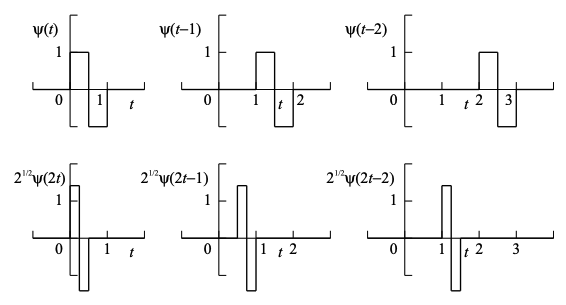
\includegraphics[height=6cm]{prml_fig_wavelet.png}
        \caption{Haar ウェーブレットの場合の関数 $\psi_{0,0} = \psi, \psi_{0,1}, \psi_{0,2}, \psi_{1,0}, \psi_{1,1}, \psi_{1,2}$}
        \label{fig:wavelet}
    \end{figure}
\end{frame}

\section{最尤推定と最小二乗法}

\begin{frame}{最尤推定と最小二乗法の関係}
    以後の議論は基底関数の形に依らないため,基底関数は特に限定しないことにする.\\
    また,簡単のため,目標変数 $t$ が1次元の場合を扱う (多次元の場合は 3.1.5 節).\\
    \vspace{11pt}
    ここでは,1章の多項式フィッティングで扱った,最小二乗法と最尤推定との関係をより詳細に議論する.\\
    1章で見たように,多項式回帰において二乗和誤差関数を最小化するパラメータ $\bs{w}$ は,ガウスノイズモデルの下での最尤推定解と一致する:
    \begin{equation}
        t = \underset{\text{deterministic}}{y(\bs{x},\bs{w})} + \underset{\text{stochastic}}{\varepsilon}, \quad \text{where} \quad \varepsilon \sim \CN(0,\sigma^{2}).
    \end{equation}
    すなわち,目標変数 $t$ の予測分布は,精度パラメータ $\beta$ を用いて,
    \begin{equation}
        p(t \mid \bs{x},\bs{w},\beta) = \CN(t \mid y(\bs{x},\bs{w}), \beta^{-1}), \quad \text{where} \quad \beta^{-1} = \sigma^{2}
    \end{equation}
    で与えられる.
\end{frame}

\begin{frame}{最尤推定と最小二乗法の関係}
    1.5.5 節で見たように,二乗損失関数を仮定すれば,入力 $\bs{x}$ の値に対する最適な予測値は目標変数の条件付き期待値
    \begin{equation}
        \BE[t \mid \bs{x}] = \int_{\BR} tp(t \mid \bs{x})dt = \int_{\BR} t\CN(t \mid y(\bs{x},\bs{w}), \beta^{-1})dt = y(\bs{x},\bs{w})
    \end{equation}
    で与えられる.
    \begin{rmk}
        ガウスノイズの仮定は,条件付き分布 $p(t \mid \bs{x})$ が単峰性のため,応用場面によっては不適切である可能性がある.
    \end{rmk}
    $\longrightarrow$ 14.5.1 節で条件付きガウス混合分布への拡張を議論 (多峰性の条件付き分布)
\end{frame}

\begin{frame}{最尤推定と最小二乗法の関係}
    最尤推定により,予測分布 $p(t \mid \bs{x},\bs{w},\beta)$ のパラメータ $\bs{w},\beta$ を推定する.\\
    入力 $\mb{X} = \{\bs{x}_{1},\ldots,\bs{x}_{N}\}$ と対応する目標値 $t_{1},\ldots,t_{N}$ からなるデータ集合を考え,$\tb{\ts{t}} = (t_{1},\ldots,t_{N})^{\top}$ とする.各データ点が分布 $\CN(t \mid y(\bs{x},\bs{w}), \beta^{-1})$ から独立に生成されたと仮定すると,尤度関数は,
    \begin{equation}
        p(\tb{\ts{t}} \mid \mb{X},\bs{w},\beta) = \prod_{n=1}^{N} \CN(t_{n} \mid y(\bs{x}_{n},\bs{w}), \beta^{-1}) = \prod_{n=1}^{N} \CN(t_{n} \mid \bs{w}^{\top}\bs{\phi}(\bs{x}_{n}),\beta^{-1})
    \end{equation}
    で与えられる.\\
    教師あり学習問題では,入力変数の分布をモデル化しないため,$\bs{x}$ は条件としてしか現れないので,以後は尤度関数の表記から $\bs{x}$ を省略して $p(\tb{\ts{t}} \mid \bs{w},\beta)$ と書く.
\end{frame}

\begin{frame}{最尤推定と最小二乗法の関係}
    このとき,対数尤度関数は,
    \begin{align}
        \ln p(\tb{\ts{t}} \mid \bs{w},\beta) &= \ln \prod_{n=1}^{N} \CN(t_{n} \mid \bs{w}^{\top}\bs{\phi}(\bs{x}_{n}),\beta^{-1}) = \sum_{n=1}^{N} \ln \CN(t_{n} \mid \bs{w}^{\top}\bs{\phi}(\bs{x}_{n}),\beta^{-1}) \\
        &= \sum_{n=1}^{N} \ln \left(\frac{1}{(2\pi\beta^{-1})^{1/2}} \exp\left(-\frac{(t_{n} - \bs{w}^{\top}\bs{\phi}(\bs{x}_{n}))^{2}}{2\beta^{-1}}\right)\right) \\
        &= \sum_{n=1}^{N} \left(\frac{1}{2} \ln \beta - \frac{1}{2} \ln (2\pi) - \beta \frac{1}{2} (t_{n} - \bs{w}^{\top}\bs{\phi}(\bs{x}_{n}))^{2}\right) \\
        &= \frac{N}{2} \ln \beta - \frac{N}{2} \ln (2\pi) - \beta \underbrace{\frac{1}{2} \sum_{n=1}^{N} (t_{n} - \bs{w}^{\top}\bs{\phi}(\bs{x}_{n}))^{2}}_{E_{D}(\bs{w}):\ \text{sum-of-squares error}} \label{eq:log likelihood function}
    \end{align}
    となる.最尤推定解を得るには,これを $\bs{w}$ と $\beta$ について最大化すればよい.
\end{frame}

\begin{frame}{最尤推定と最小二乗法の関係}
    式 \eqref{eq:log likelihood function} より,パラメータ $\bs{w}$ に関する対数尤度関数 $\ln p(\tb{\ts{t}} \mid \bs{w},\beta)$ の最大化は,二乗和誤差関数 $E_{D}(\bs{w})$ の最小化と等価である.
    \begin{itemize}
        \item ガウスノイズモデル下の最尤推定と最小二乗法との等価性
    \end{itemize}
    ここで,以下で与えられる\underline{計画行列} (design matrix)
    \begin{equation}
        \bs{\Phi} = \begin{pmatrix}
            \phi_{0}(\bs{x}_{1}) & \phi_{1}(\bs{x}_{1}) & \cdots & \phi_{M-1}(\bs{x}_{1}) \\
            \phi_{0}(\bs{x}_{2}) & \phi_{1}(\bs{x}_{2}) & \cdots & \phi_{M-1}(\bs{x}_{2}) \\
            \vdots & \vdots & \ddots & \vdots \\
            \phi_{0}(\bs{x}_{N}) & \phi_{1}(\bs{x}_{N}) & \cdots & \phi_{M-1}(\bs{x}_{N})
        \end{pmatrix} \in \BR^{N \times M}
    \end{equation}
    を考えると,二乗和誤差関数 $E_{D}(\bs{w})$ は
    \begin{equation}
        E_{D}(\bs{w}) = \frac{1}{2} \sum_{n=1}^{N} (t_{n} - \bs{w}^{\top}\bs{\phi}(\bs{x}_{n}))^{2} = \frac{1}{2} (\tb{\ts{t}} - \bs{\Phi}\bs{w})^{\top} (\tb{\ts{t}} - \bs{\Phi}\bs{w}).
    \end{equation}
\end{frame}

\begin{frame}{パラメータ $\bs{w}$ に関する対数尤度関数 $\ln p(\tb{\ts{t}} \mid \bs{w},\beta)$ の最大化}
    \vspace{-22pt}
    \begin{align}
        E_{D}(\bs{w}) &= \frac{1}{2} (\tb{\ts{t}} - \bs{\Phi}\bs{w})^{\top} (\tb{\ts{t}} - \bs{\Phi}\bs{w}) = \frac{1}{2} \left(\tb{\ts{t}}^{\top} \tb{\ts{t}} - \tb{\ts{t}}^{\top} \bs{\Phi} \bs{w} - \bs{w}^{\top} \bs{\Phi}^{\top} \tb{\ts{t}} + \bs{w}^{\top} \bs{\Phi}^{\top} \bs{\Phi} \bs{w}\right) \\
        &= \frac{1}{2} \left(\bs{w}^{\top} \bs{\Phi}^{\top} \bs{\Phi} \bs{w} - 2 \tb{\ts{t}}^{\top} \bs{\Phi} \bs{w} + \tb{\ts{t}}^{\top} \tb{\ts{t}}\right)
    \end{align}
    であり,
    \begin{enumerate}[(1)]
        \item $\bs{\Phi}^{\top} \bs{\Phi}$ は対称 $\left(\because \left(\bs{\Phi}^{\top} \bs{\Phi}\right)^{\top} = \bs{\Phi}^{\top} \left(\bs{\Phi}^{\top}\right)^{\top} = \bs{\Phi}^{\top} \bs{\Phi}\right)$,
        \item $\bs{\Phi}^{\top} \bs{\Phi}$ はグラム行列\footnote{\url{https://mathlandscape.com/gram-matrix/}} $\Longrightarrow \bs{\Phi}^{\top} \bs{\Phi} \succeq 0$,
    \end{enumerate}
    ゆえ,$E_{D}(\bs{w})$ の $\bs{w}$ に関する最小化は制約なし凸2次計画問題\footnote{\url{http://www.me.titech.ac.jp/~mizu_lab/lib/pdf/kougisiryou/suuti/handout/11/suuti_kougi11-6.pdf}}なので,
    \begin{equation}
        \bs{w}_{\text{ML}} = \argmin_{\bs{w} \in \BR^{M}} E_{D}(\bs{w}) \iff \left.\frac{\partial}{\partial{\bs{w}}} E_{D}(\bs{w})\right|_{\bs{w} = \bs{w}_{\text{ML}}} = 0.
    \end{equation}
\end{frame}

\begin{frame}{パラメータ $\bs{w}$ に関する対数尤度関数 $\ln p(\tb{\ts{t}} \mid \bs{w},\beta)$ の最大化}
    \vspace{-22pt}
    \begin{align}
        \frac{\partial}{\partial{\bs{w}}} \ln p(\tb{\ts{t}} \mid \bs{w},\beta) &= \frac{\partial}{\partial{\bs{w}}} \left(-\beta E_{D}(\bs{w})\right) = - \frac{\beta}{2} \frac{\partial}{\partial{\bs{w}}} (\tb{\ts{t}} - \bs{\Phi}\bs{w})^{\top} (\tb{\ts{t}} - \bs{\Phi}\bs{w}) \\
        &= -\frac{\beta}{2} \frac{\partial}{\partial{\bs{w}}} \left(\bs{w}^{\top} \bs{\Phi}^{\top} \bs{\Phi} \bs{w} - 2 \tb{\ts{t}}^{\top} \bs{\Phi} \bs{w} + \tb{\ts{t}}^{\top} \tb{\ts{t}} \right) \\
        &= - \frac{\beta}{2} \left(2 \bs{\Phi}^{\top} \bs{\Phi} \bs{w} - 2 \bs{\Phi}^{\top} \tb{\ts{t}}\right) = - \beta \left(\bs{\Phi}^{\top} \bs{\Phi} \bs{w} - \bs{\Phi}^{\top} \tb{\ts{t}}\right) \\
        & \qquad \left(\because \frac{\partial}{\partial{\bs{w}}} \bs{w}^{\top} \mb{A} \bs{w} = (\mb{A} + \mb{A}^{\top}) \bs{w}, \quad \frac{\partial}{\partial{\bs{w}}} \bs{a}^{\top} \bs{w} = \bs{a} \right)
    \end{align}
    ゆえ,\underline{$\bs{\Phi}^{\top}\bs{\Phi}$ が正則ならば},最尤推定解 $\bs{w}_{\text{ML}}$ は,
    \begin{align}
        \left.\frac{\partial}{\partial{\bs{w}}} \ln p(\tb{\ts{t}} \mid \bs{w},\beta)\right|_{\bs{w} = \bs{w}_{\text{ML}}} = 0 &\iff \bs{\Phi}^{\top} \bs{\Phi} \bs{w}_{\text{ML}} - \bs{\Phi}^{\top} \tb{\ts{t}} = 0 \label{eq:maximum likelihood} \\
        &\iff \bs{w}_{\text{ML}} = \left(\bs{\Phi}^{\top}\bs{\Phi}\right)^{-1} \bs{\Phi}^{\top} \tb{\ts{t}}. \label{eq:normal equation}
    \end{align}
\end{frame}

\begin{frame}{パラメータ $\bs{w}$ に関する対数尤度関数 $\ln p(\tb{\ts{t}} \mid \bs{w},\beta)$ の最大化}
    \begin{itemize}
        \item 方程式 \eqref{eq:normal equation} を最小二乗問題の\underline{正規方程式} (normal equation) という.
        \item 行列 $\bs{\Phi}^{\dagger} \equiv \left(\bs{\Phi}^{\top}\bs{\Phi}\right)^{-1} \bs{\Phi}^{\top} \in \BR^{M \times N}$ を行列 $\bs{\Phi}$ の\underline{ムーア-ペンローズの擬似逆行列}\footnote{\url{https://ja.wikipedia.org/wiki/\%E3\%83\%A0\%E3\%83\%BC\%E3\%82\%A2\%E3\%83\%BB\%E3\%83\%9A\%E3\%83\%B3\%E3\%83\%AD\%E3\%83\%BC\%E3\%82\%BA\%E9\%80\%86\%E8\%A1\%8C\%E5\%88\%97}} (Moore-Penrose pseudo-inverse matrix) という.
        \begin{itemize}
            \item[-] 通常の逆行列の概念の非正方行列への拡張
            \item[-] 実際,$\bs{\Phi}$ が正則ならば,$\bs{\Phi}^{-1}$ が存在し,
            \begin{equation}
                \bs{\Phi}^{\dagger} \equiv \left(\bs{\Phi}^{\top}\bs{\Phi}\right)^{-1} \bs{\Phi}^{\top} = \bs{\Phi}^{-1} \left(\bs{\Phi}^{\top}\right)^{-1} \bs{\Phi}^{\top} = \bs{\Phi}^{-1}.
            \end{equation}
            \item[-] 任意の行列 $\mb{M}$ に対して,定義の4条件を満たす擬似逆行列 $\mb{M}^{\dagger}$ が一意に存在
        \end{itemize}
        \item 式 \eqref{eq:maximum likelihood} において $\bs{\Phi}^{\top}\bs{\Phi}$ が正則でない場合については後述.
        \begin{itemize}
            \item[-] 計画行列 $\bs{\Phi}$ がフルランクでない場合に発生する (\underline{多重共線性}\footnote{\url{https://ja.wikipedia.org/wiki/\%E5\%A4\%9A\%E9\%87\%8D\%E5\%85\%B1\%E7\%B7\%9A\%E6\%80\%A7}} (Multicollinearity)).
        \end{itemize}
    \end{itemize}
\end{frame}

\begin{frame}{パラメータ $\beta$ に関する対数尤度関数 $\ln p(\tb{\ts{t}} \mid \bs{w}_{\text{ML}},\beta)$ の最大化}
    次に,パラメータ $\beta$ に関して対数尤度関数 $\ln p(\tb{\ts{t}} \mid \bs{w}_{\text{ML}},\beta)$ を最大化する.
    \begin{align}
        \frac{\partial}{\partial{\beta}} \ln p(\tb{\ts{t}} \mid \bs{w}_{\text{ML}},\beta) &= \frac{\partial}{\partial{\beta}} \left(\frac{N}{2} \ln \beta - \frac{N}{2} \ln (2\pi) - \beta \frac{1}{2} \sum_{n=1}^{N} (t_{n} - \bs{w}_{\text{ML}}^{\top}\bs{\phi}(\bs{x}_{n}))^{2}\right) \\
        &= \frac{N}{2} \frac{1}{\beta} - \frac{1}{2} \sum_{n=1}^{N} (t_{n} - \bs{w}_{\text{ML}}^{\top}\bs{\phi}(\bs{x}_{n}))^{2}
    \end{align}
    ゆえ,最尤推定解 $\beta_{\text{ML}}$ は,
    \begin{equation}
        \left.\frac{\partial}{\partial{\beta}} \ln p(\tb{\ts{t}} \mid \bs{w}_{\text{ML}},\beta)\right|_{\beta = \beta_{\text{ML}}} = 0 \iff \frac{1}{\beta_{\text{ML}}} = \frac{1}{N} \sum_{n=1}^{N} (\underbrace{t_{n} - \bs{w}_{\text{ML}}^{\top}\bs{\phi}(\bs{x}_{n})}_{\text{residual}})^{2}
    \end{equation}
    として得られ,$\beta_{\text{ML}}^{-1} = \sigma_{\text{ML}}^{2}$ は回帰関数 $y(\bs{x},\bs{w}_{\text{ML}})$ 周りでの目標値の残差分散で与えられることがわかる.
\end{frame}

\begin{frame}{バイアスパラメータ $w_{0}$ の役割}
    二乗和誤差関数 $E_{D}(\bs{w})$ において,バイアスパラメータ $w_{0}$ を明示的に書くと,
    \begin{gather}
        E_{D}(\bs{w}) = \frac{1}{2} \sum_{n=1}^{N} (t_{n} - \bs{w}^{\top}\bs{\phi}(\bs{x}_{n}))^{2} = \frac{1}{2} \sum_{n=1}^{N} \left(t_{n} - w_{0} - \sum_{j=1}^{M-1} w_{j} \phi_{j}(\bs{x}_{n})\right)^{2} \\
        \Longrightarrow \frac{\partial}{\partial{w_{0}}} E_{D}(\bs{w}) = - \sum_{n=1}^{N} \left(t_{n} - w_{0} - \sum_{j=1}^{M-1} w_{j} \phi_{j}(\bs{x}_{n})\right)
    \end{gather}
    ゆえ,$E_{D}(\bs{w})$ を最小化するパラメータ $\hat{w}_{0}$ は,
    \begin{equation}
        \left.\frac{\partial}{\partial{w_{0}}} E_{D}(\bs{w})\right|_{w_{0} = \hat{w}_{0}} = 0 \iff \hat{w}_{0} = \textcolor{red}{\frac{1}{N} \sum_{n=1}^{N} t_{n}} - \sum_{j=1}^{M-1} w_{j} \left(\textcolor{blue}{\frac{1}{N} \sum_{n=1}^{N} \phi_{j}(\bs{x}_{n})}\right) \equiv \textcolor{red}{\overline{t}} - \sum_{j=1}^{M-1} w_{j} \textcolor{blue}{\overline{\phi_{j}}}.
    \end{equation}
    バイアスパラメータ $w_{0}$ は,訓練データ $\{(\bs{x}_{n}, t_{n})\}_{n=1}^{N}$ に関する,目標値の平均 $\overline{t}$ と,基底関数の値の平均の重み付き和 $\sum_{j=1}^{M-1} w_{j} \overline{\phi_{j}}$ との差を埋め合わせる役割をしている.
\end{frame}

\section{最小二乗法の幾何学}

\begin{frame}{最小二乗解の幾何学的解釈}
    計画行列 $\bs{\Phi}$ の第 $j$ 列を $\bs{\varphi}_{j} = (\phi_{j-1}(\bs{x}_{1}),\ldots,\phi_{j-1}(\bs{x}_{N}))^{\top} \in \BR^{N}$ とおくと,
    \begin{equation}
        \bs{\Phi} = \begin{pmatrix}
            \phi_{0}(\bs{x}_{1}) & \phi_{1}(\bs{x}_{1}) & \cdots & \phi_{M-1}(\bs{x}_{1}) \\
            \phi_{0}(\bs{x}_{2}) & \phi_{1}(\bs{x}_{2}) & \cdots & \phi_{M-1}(\bs{x}_{2}) \\
            \vdots & \vdots & \ddots & \vdots \\
            \phi_{0}(\bs{x}_{N}) & \phi_{1}(\bs{x}_{N}) & \cdots & \phi_{M-1}(\bs{x}_{N})
        \end{pmatrix} = \begin{pmatrix}
            \bs{\varphi}_{1} & \bs{\varphi}_{2} & \cdots & \bs{\varphi}_{M}
        \end{pmatrix} \in \BR^{N \times M}.
    \end{equation}
    このとき,基底関数の数 $M$ がデータ点数 $N$ よりも小さければ\footnote{$M \ge N$ かつ $\bs{\Phi}$ がフルランクならば $\CS = \BR^{N}$.},$M$ 個のベクトル $\{\bs{\varphi}_{j}\}_{j=1}^{M}$ は $M$ 次元線形部分空間 $\CS \subsetneq \BR^{N}$ を張る:
    \begin{equation}
        \CS = \text{Im}\, \bs{\Phi} = \text{span}_{\BR}(\bs{\varphi}_{1},\ldots,\bs{\varphi}_{M}) = \left\{\sum_{j=1}^{M} w_{j} \bs{\varphi}_{j} \ \middle|\ \bs{w} \in \BR^{M}\right\} \subsetneq \BR^{N}.
    \end{equation}    
\end{frame}

\begin{frame}{最小二乗解の幾何学的解釈}
    ベクトル $\tb{\ts{y}} \in \BR^{N}$ を
    \begin{equation}
        \tb{\ts{y}} \coloneqq (y(\bs{x}_{1},\bs{w}),\ldots,y(\bs{x}_{N},\bs{w}))^{\top}
    \end{equation}
    で定義すると,$y(\bs{x}_{n},\bs{w}) = \bs{w}^{\top} \bs{\phi}(\bs{x}_{n})$ より,
    \begin{equation}
        \tb{\ts{y}} = (\bs{w}^{\top} \bs{\phi}(\bs{x}_{1}),\ldots,\bs{w}^{\top} \bs{\phi}(\bs{x}_{N}))^{\top} = \bs{\Phi} \bs{w} \in \CS.
    \end{equation}
    ここで,最小二乗解 $\bs{w}_{\text{ML}}$ は,$\norm{\cdot}_{2}$ をユークリッドノルムとして,
    \begin{equation}
        \bs{w}_{\text{ML}} = \argmin_{\bs{w} \in \BR^{M}} E_{D}(\bs{w}) = \argmin_{\bs{w} \in \BR^{M}} \frac{1}{2} \norm{\tb{\ts{t}} - \underbrace{\bs{\Phi}\bs{w}}_{\tb{\ts{y}}}}_{2}^{2}
    \end{equation}
    で与えられるので,最小二乗解 $\bs{w}_{\text{ML}} \in \BR^{M}$ を求めることは,ユークリッド距離で $\tb{\ts{t}} \in \BR^{N}$ に最も近い $\bs{\Phi} \bs{w} = \tb{\ts{y}} \in \CS$ を選ぶことに相当する.この $\tb{\ts{y}} \in \CS$ は,$\tb{\ts{t}} \in \BR^{N}$ の部分空間 $\CS$ 上への正射影に対応する (次ページ参照).
\end{frame}

\begin{frame}{最小二乗解の幾何学的解釈}
    \begin{columns}
        \begin{column}{0.5\textwidth}
        \underline{直観的な説明}
            \begin{itemize}
                \item $N=3,M=2$ の場合は下図
            \end{itemize}
            \begin{table}[h]
                \centering
                \begin{tabular}{ll}
                    minimize & $\displaystyle\norm{\tb{\ts{t}} - \tb{\ts{y}}}_{2}^{2}$ \\
                    subject to & $\tb{\ts{y}} \in \CS$
                \end{tabular}
            \end{table}
            \begin{figure}
                \centering
                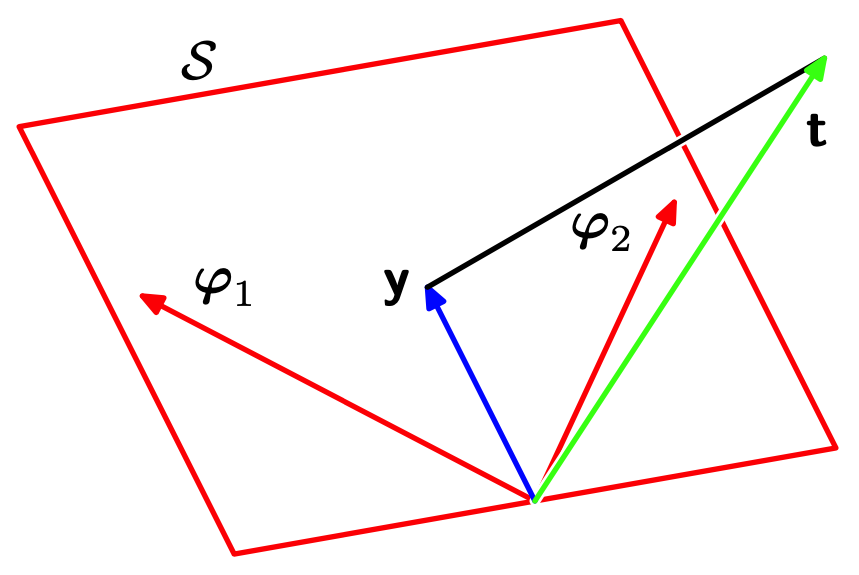
\includegraphics[height=3cm]{prml_fig_3-2.png}
                \caption{最小二乗解の幾何学的解釈}
                \label{fig:3.2}
            \end{figure}
        \end{column}
        \begin{column}{0.5\textwidth}
            \underline{理論的な説明}\\
            \vspace{2.5pt}
            行列 $\bs{\Phi} \left(\bs{\Phi}^{\top} \bs{\Phi}\right)^{-1} \bs{\Phi}^{\top}$ は任意のベクトル $\bs{v} \in \BR^{N}$ を $\CS = \text{span}_{\BR}(\bs{\varphi}_{1},\ldots,\bs{\varphi}_{M})$ に正射影する ($\because$ 演習 3.2).したがって,
            \begin{equation}
                \bs{w}_{\text{ML}} = \left(\bs{\Phi}^{\top} \bs{\Phi}\right)^{-1} \bs{\Phi}^{\top} \tb{\ts{t}}
            \end{equation}
            より,
            \begin{equation} \label{eq:projection}
                \hat{\tb{\ts{y}}} = \bs{\Phi} \bs{w}_{\text{ML}} = \bs{\Phi} \left(\bs{\Phi}^{\top} \bs{\Phi}\right)^{-1} \bs{\Phi}^{\top} \tb{\ts{t}}
            \end{equation}
            は $\tb{\ts{t}} \in \BR^{N}$ の部分空間 $\CS$ 上への正射影となっている.
        \end{column}
    \end{columns}
\end{frame}

\begin{frame}{$\bs{\Phi}^{\top} \bs{\Phi}$ が正則でない (非正則に近い) 場合の対処法}
    式 \eqref{eq:maximum likelihood} において $\bs{\Phi}^{\top} \bs{\Phi}$ が正則でない場合には,最尤推定解 $\bs{w}_{\text{ML}}$ を求められない.\\
    特に,2つ以上の基底ベクトル $\bs{\varphi}_{j}$ が線形従属の場合,$\rank \bs{\Phi} < \min (M,N)$ となり,このような問題が発生する.また,2つ以上の基底ベクトル $\bs{\varphi}_{j}$ が線形従属に近い場合にも同様の問題が発生し,求まるパラメータ $\bs{w}_{\text{ML}}$ が数値的に不安定になる.\\
    この問題の対処法として以下のような手法がある.
    \begin{itemize}
        \item 特異値分解\footnote{\url{https://ja.wikipedia.org/wiki/\%E7\%89\%B9\%E7\%95\%B0\%E5\%80\%A4\%E5\%88\%86\%E8\%A7\%A3}} (singular value decomposition; SVD)
        \begin{itemize}
            \item[-] 陽に逆行列 $\left(\bs{\Phi}^{\top} \bs{\Phi}\right)^{-1}$ を計算せずとも,擬似逆行列 $\bs{\Phi}^{\dagger}$ を計算することができる.
        \end{itemize}
        \item 正則化最小二乗法 ($\longrightarrow$ 3.1.4 節)
        \begin{itemize}
            \item[-] 正則化項を加えることにより,$\bs{\Phi}^{\top} \bs{\Phi}$ が正則でない場合でも最適解 $\bs{w}_{\text{ML}}$ が得られる.
            \item[-] 特に,$q=2$ (Ridge回帰) の場合は解析的に最適解が求められる.
        \end{itemize}
        \vspace{-17pt}
        \begin{table}[h]
                \centering
                \begin{tabular}{ccccc}
                    minimize & $\norm{\tb{\ts{t}} - \bs{\Phi} \bs{w}}_{2}^{2} + \lambda \norm{\bs{w}}_{q}^{q}$ & subject to & $\bs{w} \in \BR^{M}$,  & where $\norm{\cdot}_{q}$ is $L^{q}$-norm\footnote{\url{https://ja.wikipedia.org/wiki/Lp\%E7\%A9\%BA\%E9\%96\%93}}.
                \end{tabular}
            \end{table}
    \end{itemize}
\end{frame}

\begin{frame}{特異値分解定理}
    \footnotesize
    \begin{theorem}[特異値分解定理\footnote{証明: \url{https://qiita.com/gyu-don/items/2e4fd7e945d8c349afb5}}]
        $\mb{M} \in \BC^{m \times n}$ を $\rank \mb{M} = r$ の行列とする.このとき,$\mb{\Sigma} \in \BC^{m \times n}$ が一意に存在し,
        \begin{equation} \label{eq:SVD}
            \mb{M} = \mb{U} \mb{\Sigma} \mb{V}^{\ast}
        \end{equation}
        の分解が成り立つ.ただし,$\mb{U},\mb{V}$ はそれぞれ $m \times m$, $n \times n$ のユニタリ行列であり,$\mb{\Sigma}$ は半正定値行列 $\mb{M}\mb{M}^{\ast}$ あるいは $\mb{M}^{\ast}\mb{M}$ の正の固有値\footnote{$\mb{M}\mb{M}^{\ast}$ と $\mb{M}^{\ast}\mb{M}$ の非零固有値は一致する: \url{http://teagis.ip.is.saga-u.ac.jp/svd.pdf}}の平方根 $\sigma_{1} \ge \cdots \ge \sigma_{r} > 0$ および $q = \min(m,n),$ $\sigma_{r+1} = \cdots = \sigma_{q} = 0$ を用いて
        \begin{equation}
            \mb{\Sigma} = \begin{dcases}
                \begin{pmatrix}
                    \mb{\Delta} & \mb{O} 
                \end{pmatrix}, & (m < n),\\
                \mb{\Delta}, & (m = n), \\
                \begin{pmatrix}
                    \mb{\Delta} \\
                    \mb{O}
                \end{pmatrix}, & (m > n),
            \end{dcases} \quad \text{where} \quad \mb{\Delta} = \diag(\sigma_{1},\ldots,\sigma_{q}) = \begin{pmatrix}
                \sigma_{1} & & \mb{O} \\
                & \ddots & \\
                \mb{O} & & \sigma_{q}
            \end{pmatrix}
        \end{equation}
        で与えられる.分解 \eqref{eq:SVD} を $\mb{M}$ の\underline{特異値分解},$\sigma_{1},\ldots,\sigma_{q}$ を $\mb{M}$ の\underline{特異値}と呼ぶ.
    \end{theorem}
\end{frame}

\begin{frame}{特異値分解の計算と幾何学的解釈}
    \begin{columns}
        \begin{column}{0.5\textwidth}
            ユニタリ行列による変換は等長変換なので,特異値分解 $\mb{M} = \mb{U} \mb{\Sigma} \mb{V}^{\ast}$ におけるそれぞれの線形変換は,
            \begin{itemize}
                \item $\mb{V}^{\ast}$ : 回転 ($\because$ ユニタリ行列)
                \item $\mb{\Sigma}$ : 拡大・縮小
                \item $\mb{U}$ : 回転 ($\because$ ユニタリ行列)
            \end{itemize}
            を表す.また,$\mb{M} = \mb{U} \mb{\Sigma} \mb{V}^{\ast}$ より
            \begin{equation}
                \mb{M} \mb{M}^{\ast} = \mb{U} \mb{\Sigma} \mb{\Sigma}^{\top} \mb{U}^{\ast}, \quad \mb{M}^{\ast} \mb{M} = \mb{V} \mb{\Sigma}^{\top} \mb{\Sigma} \mb{V}^{\ast},
            \end{equation}
            ゆえ,特異値分解における $\mb{U},\mb{V}$ はそれぞれ $\mb{M} \mb{M}^{\ast}, \mb{M}^{\ast} \mb{M}$ の固有値分解によって得られる.
        \end{column}
        \begin{column}{0.5\textwidth}
            \begin{figure}
                \centering
                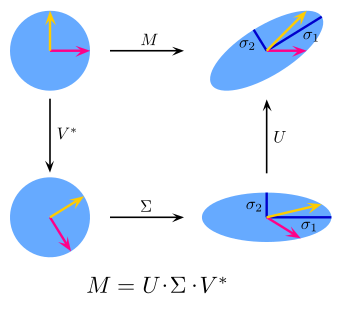
\includegraphics[height=6cm]{SVD.png}
                \caption{特異値分解の図示}
                \label{fig:SVD}
            \end{figure}
        \end{column}
    \end{columns}
\end{frame}

\begin{frame}{特異値分解による擬似逆行列 $\bs{\Phi}^{\dagger}$ の計算}
    特異値分解定理により,計画行列 $\bs{\Phi} \in \BR^{N \times M}$ に対して,直交行列 $\mb{U} \in \BR^{N \times N}$, $\mb{V} \in \BR^{M \times M}$ および行列 $\mb{\Sigma} \in \BR^{N \times M}$ が存在し,$\bs{\Phi} = \mb{U} \mb{\Sigma} \mb{V}^{\top}$ の分解が成り立つ.\\
    いま,$\mb{U},\mb{V}$ は直交行列ゆえ,
    \begin{equation}
        \mb{U}\mb{U}^{\top} = \mb{U}^{\top}\mb{U} = \mb{I}, \quad \mb{V}\mb{V}^{\top} = \mb{V}^{\top}\mb{V} = \mb{I}, \quad \mb{U}^{-1} = \mb{U}^{\top}, \quad \mb{V}^{-1} = \mb{V}^{\top}
    \end{equation}
    が成り立つことに注意すると,
    \begin{align}
        \bs{\Phi}^{\dagger} &= \left(\bs{\Phi}^{\top}\bs{\Phi}\right)^{-1} \bs{\Phi}^{\top} = \left(\mb{V} \mb{\Sigma}^{\top} \mb{U}^{\top} \mb{U} \mb{\Sigma} \mb{V}^{\top}\right)^{-1} \mb{V} \mb{\Sigma}^{\top} \mb{U}^{\top} \\
        &= \mb{V} \left(\mb{\Sigma}^{\top} \mb{\Sigma}\right)^{-1} \mb{V}^{\top} \mb{V} \mb{\Sigma}^{\top} \mb{U}^{\top} = \mb{V} \left(\mb{\Sigma}^{\top} \mb{\Sigma}\right)^{-1} \mb{\Sigma}^{\top} \mb{U}^{\top} \\
        &\equiv \mb{V} \mb{\Sigma}^{\dagger} \mb{U}^{\top}. \qquad (\mb{\Sigma}^{\dagger} \in \BR^{M \times N})
    \end{align}
    \vspace{11pt}
    ただし,$\mb{\Sigma}^{\dagger} \equiv \left(\mb{\Sigma}^{\top} \mb{\Sigma}\right)^{-1} \mb{\Sigma}^{\top}$ は,$\mb{\Sigma}$ の非零成分\footnote{数値計算では,許容誤差よりも大きい要素のみが非零と見なされ,他の要素は0に置き換えられる.}の逆数を成分とする行列の転置.
\end{frame}

\section{まとめ}

\begin{frame}{まとめ}
    \begin{itemize}
        \item 線形基底関数モデル
        \begin{itemize}
            \item[-] 基底関数 $\phi_{j}$ からなる特徴写像 $\bs{\phi}$ によって線形回帰モデルを拡張
            \item[-] 様々な基底関数が使われる
        \end{itemize}
        \item 最尤推定と最小二乗法
        \begin{itemize}
            \item[-] 最小二乗解とガウスノイズモデル下の最尤推定解は一致
            \item[-] 計画行列 $\bs{\Phi}$ がフルランクならば,最小二乗解 $\bs{w}_{\text{ML}}$ は解析的に求められる
        \end{itemize}
        \item 最小二乗法の幾何学
        \begin{itemize}
            \item[-] 最小二乗解 $\bs{w}_{\text{ML}}$ の求解は,訓練データの目標値からなるベクトル $\tb{\ts{t}} \in \BR^{N}$ のモデル空間 $\CS = \text{Im}\, \bs{\Phi} = \text{span}_{\BR}(\bs{\varphi}_{1},\ldots,\bs{\varphi}_{M})$ 上への正射影を求めることに対応する
            \item[-] $\bs{\Phi}^{\top} \bs{\Phi}$ が非正則に近い場合の対処法
            \begin{itemize}
                \item[*] 特異値分解
                \item[*] 正則化最小二乗法
                \item[*] 正則化の一種として,主成分回帰\footnote{\url{https://en.wikipedia.org/wiki/Principal_component_regression}} (principal component regression; PCR) などもある
            \end{itemize}
        \end{itemize}
    \end{itemize}
\end{frame}

\section{演習問題 (Appendix)}

\begin{frame}{演習問題 (Appendix)}
    \fontsize{6.5pt}{0cm}\selectfont
    \begin{block}{演習 3.1 (基本) \fbox{www}}
        $\tanh$ 関数とロジスティックシグモイド関数は次のように関係付けられることを示せ.
        \begin{equation} \label{eq:tanh and logistic sigmoid}
            \tanh(a) = 2\sigma(2a) - 1.
        \end{equation}
        さらに,次の形のロジスティックシグモイド関数の線形結合
        \begin{equation}
            y(x,\bs{w}) = w_{0} + \sum_{j=1}^{M} w_{j} \sigma\left(\frac{x-\mu_{j}}{s}\right)
        \end{equation}
        は次の形の $\tanh$ 関数の線形結合
        \begin{equation}
            y(x,\bs{u}) = u_{0} + \sum_{j=1}^{M} u_{j} \tanh\left(\frac{x-\mu_{j}}{2s}\right)
        \end{equation}
        と等価であることを示し,新しいパラメータ $\{u_{0},\ldots,u_{M}\}$ ともとのパラメータ $\{w_{0},\ldots,w_{M}\}$ を関係付ける式を求めよ.
    \end{block}
    (解答) 式 \eqref{eq:tanh} より,式 \eqref{eq:tanh and logistic sigmoid} が成り立つ.これを用いると,
    \begin{equation}
        y(x,\bs{u}) = u_{0} + \sum_{j=1}^{M} u_{j} \tanh\left(\frac{x-\mu_{j}}{2s}\right) = u_{0} + \sum_{j=1}^{M} u_{j} \left\{2\sigma\left(\frac{x-\mu_{j}}{s}\right) - 1\right\} = u_{0} - \sum_{j=1}^{M} u_{j} + \sum_{j=1}^{M} 2 u_{j} \sigma\left(\frac{x-\mu_{j}}{s}\right)
    \end{equation}
    ゆえ,パラメータの関係式は $w_{0} = u_{0} - \sum_{j=1}^{M} u_{j},\ w_{j} = 2 u_{j}\ (j=1,\ldots,M)$ で与えられる.
\end{frame}

\begin{frame}{演習問題 (Appendix)}
    \fontsize{7pt}{0cm}\selectfont
    \begin{block}{演習 3.2 (標準)}
        行列
        \begin{equation}
            \bs{\Phi} \left(\bs{\Phi}^{\top} \bs{\Phi}\right)^{-1} \bs{\Phi}^{\top}
        \end{equation}
        は任意のベクトル $\bs{v}$ を $\bs{\Phi}$ の列ベクトルで張られる空間の上に正射影することを示せ.そしてこの結果を使って,最小二乗解 \eqref{eq:normal equation} は図 \ref{fig:3.2} で示した多様体 $\CS$ の上にベクトル $\tb{\ts{t}}$ を正射影することに対応していることを示せ.
    \end{block}
    (解答) 行列 $\bs{\Phi} = \left(\bs{\varphi}_{1},\ldots,\bs{\varphi}_{M}\right) \in \BR^{N \times M}$ に対して,部分空間 $\CS \in \BR^{N}$ を $\CS = \text{span}_{\BR}\left(\bs{\varphi}_{1},\ldots,\bs{\varphi}_{M}\right)$ とおく.任意のベクトル $\bs{v} \in \BR^{N}$ の $\CS$ 上への正射影 $\bs{p}$ は,$\bs{w} = (w_{1},\ldots,w_{M}) \in \BR^{M}$ を用いて,$\bs{p} = \sum_{j=1}^{M} w_{j} \bs{\varphi}_{j} = \bs{\Phi} \bs{w}$ と表せる.このとき,ベクトル $\bs{v} - \bs{p}$ と $\CS$ の基底 $\bs{\varphi}_{1},\ldots,\bs{\varphi}_{M}$ は直交するので,
    \begin{align}
        \ip{\bs{v} - \bs{p}, \bs{\varphi}_{j}} = 0, \quad \forall j \in \{1,\ldots,M\} &\iff \bs{\Phi}^{\top} (\bs{v} - \bs{p}) = 0 \\
        &\iff \bs{\Phi}^{\top} (\bs{v} - \bs{\Phi} \bs{w}) = 0 \\
        &\iff \bs{w} = \left(\bs{\Phi}^{\top} \bs{\Phi}\right)^{-1} \bs{\Phi}^{\top} \bs{v}
    \end{align}
    が成り立つ.したがって,$\bs{v}$ の正射影 $\bs{p}$ は,
    \begin{equation}
        \bs{p} = \bs{\Phi} \bs{w} = \bs{\Phi} \left(\bs{\Phi}^{\top} \bs{\Phi}\right)^{-1} \bs{\Phi}^{\top} \bs{v}
    \end{equation}
    で表されるので,行列 $\bs{\Phi} \left(\bs{\Phi}^{\top} \bs{\Phi}\right)^{-1} \bs{\Phi}^{\top}$ は任意のベクトル $\bs{v}$ を $\bs{\Phi}$ の列ベクトルで張られる空間の上に正射影する.最小二乗解 \eqref{eq:normal equation} が多様体 $\CS$ の上にベクトル $\tb{\ts{t}}$ を正射影することに対応していることは,式 \eqref{eq:projection} より成り立つ.\qed
\end{frame}

\begin{frame}{演習問題 (Appendix)}
    \fontsize{7pt}{0cm}\selectfont
    \begin{block}{演習 3.3 (基本)}
        それぞれのデータ点 $t_{n}$ に重み要素 $r_{n} > 0$ が割り当てられており,二乗和誤差関数が
        \begin{equation}
            E_{D}(\bs{w}) = \frac{1}{2} \sum_{n=1}^{N} r_{n} \left\{t_{n} - \bs{w}^{\top} \bs{\phi}(\bs{x}_{n})\right\}^{2}
        \end{equation}
        となるデータ集合を考える.このとき,この誤差関数を最小にする解 $\bs{w}^{\ast}$ についての式を求めよ.また,(i) ノイズの分散がデータに依存する場合,(ii) データ点に重複がある場合に照らして,それぞれ重み付き二乗和誤差関数の解釈を与えよ.
    \end{block}
    (解答) 行列 $\mb{R}$ を $\mb{R} = \diag(r_{1},\ldots,r_{N}) \in \BR^{N \times N}$ とすると,
    \begin{align}
        E_{D}(\bs{w}) &= \frac{1}{2} \sum_{n=1}^{N} r_{n} \left\{t_{n} - \bs{w}^{\top} \bs{\phi}(\bs{x}_{n})\right\}^{2} = \frac{1}{2} (\tb{\ts{t}} - \bs{\Phi} \bs{w})^{\top} \mb{R} (\tb{\ts{t}} - \bs{\Phi} \bs{w}) \\
        &= \frac{1}{2} (\tb{\ts{t}}^{\top} - \bs{w}^{\top} \bs{\Phi}^{\top}) \mb{R} (\tb{\ts{t}} - \bs{\Phi} \bs{w}) = \frac{1}{2} (\bs{w}^{\top} \bs{\Phi}^{\top} \mb{R} \bs{\Phi} \bs{w} - 2 \tb{\ts{t}}^{\top} \mb{R} \bs{\Phi} \bs{w} + \tb{\ts{t}}^{\top} \mb{R} \tb{\ts{t}})
    \end{align}
    ゆえ,
    \begin{equation}
        \frac{\partial}{\partial{\bs{w}}} E_{D}(\bs{w}) = \bs{\Phi}^{\top} \mb{R} \bs{\Phi} \bs{w} - \bs{\Phi}^{\top} \mb{R} \tb{\ts{t}} \quad \Longrightarrow \quad \left.\frac{\partial}{\partial{\bs{w}}} E_{D}(\bs{w})\right|_{\bs{w} = \bs{w}^{\ast}} = 0 \iff \bs{w}^{\ast} = \left(\bs{\Phi}^{\top} \mb{R} \bs{\Phi}\right)^{-1} \bs{\Phi}^{\top} \mb{R} \tb{\ts{t}}.
    \end{equation}
\end{frame}

\begin{frame}{演習問題 (Appendix)}
    \fontsize{7pt}{0cm}\selectfont
    \begin{block}{演習 3.3 (基本)}
        それぞれのデータ点 $t_{n}$ に重み要素 $r_{n} > 0$ が割り当てられており,二乗和誤差関数が
        \begin{equation}
            E_{D}(\bs{w}) = \frac{1}{2} \sum_{n=1}^{N} r_{n} \left\{t_{n} - \bs{w}^{\top} \bs{\phi}(\bs{x}_{n})\right\}^{2}
        \end{equation}
        となるデータ集合を考える.このとき,この誤差関数を最小にする解 $\bs{w}^{\ast}$ についての式を求めよ.また,(i) ノイズの分散がデータに依存する場合,(ii) データ点に重複がある場合に照らして,それぞれ重み付き二乗和誤差関数の解釈を与えよ.
    \end{block}
    (解答続き) (i) ノイズの分散がデータに依存する場合,式 \eqref{eq:log likelihood function} より,重み付き二乗和誤差関数はデータ点 $t_{n}$ のノイズの分散が $r_{n}^{-1}$ で与えられている場合の二乗和誤差関数と解釈できる.(ii) データ点に重複がある場合,重み付き二乗和誤差関数はデータ点 $(\bs{x}_{n},t_{n})$ が $r_{n}$ 個重複している場合の二乗和誤差関数と解釈できる.
\end{frame}

\end{document}